\chapter{Implementation}
\section{Potential fields}
The potential fields control algorithm simulation was implemented inside MATLAB, as described above. It is capable of successfully leading n-number of robots from the start position to the goal, assuming that the wheeled mobile robots move in the horizontal plane. Due to hardware limitations, the Khepera robots were only used to simulate the potential field control algorithm. The robot's lack the ability to traverse rough terrain, therefore the high speed convoying and rough terrain navigation was simulated through MATLAB. A screen capture of the algorithm in progress can be seen in figure \ref{fig:pot_fields_imp}. Three robots are shown avoiding a simple obstacle (in this particular situation, a chair.) The background shows the gradient representation of the goal potential field (located slightly north of the chair.) Blue represents the lowest areas of the gradient, and red the highest. In this particular run, the objects have a very narrow and tall field around them.

\begin{figure}[t]
	\centering
	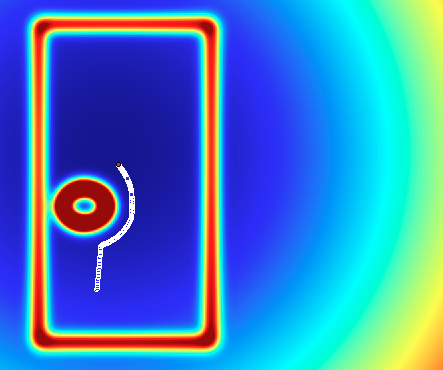
\includegraphics[width=0.8\textwidth]{figures/pot_fields_imp.png}
	\caption{A screen capture of the potential fields control simulation}
	\label{fig:pot_fields_imp}
\end{figure}

\section{Dynamics}
A simulation of the robot was created in MATLAB using the derived dynamics. A terrain was given as input, and the robot was simulated driving over it, returning the state of it's centers of mass. To calculate the state, the ode45 solver in MATLAB was used to iterate over the full version of the characteristic equation \eqref{eq:car_characteristic}. This gave access to the full state of the centers of mass, namely the accelerations, velocities, and positions of the body center of mass, tire centers of mass, and the body angles.

Following this, a second robot was simulated driving a fixed distance behind the first one and matching the speed, as shown in figure \ref{fig:naive_convoy}. It recorded the changes in position, velocity, and acceleration of the body center of mass of the vehicle in front. Because the system is not rigid, the dynamics depend on the position of the wheels. However, this data would not be able to be recorded outside of a simulation. To account for this, the following robot runs the dynamics on the last state of the lead robot in an attempt to guess the current location of the wheels. The estimated wheel states from the last time step are combined with the real body states from the current time step to create an estimation of the change in ground height under the lead vehicle.

\begin{figure}[t]
	\centering
	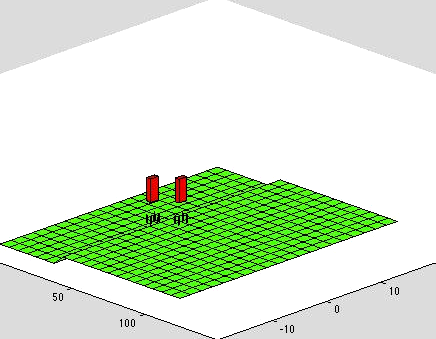
\includegraphics[width=0.8\textwidth]{figures/naive_convoy.png}
	\caption{A screen capture of the convoy approaching a bump.}
	\label{fig:naive_convoy}
\end{figure}

A steering model was then implemented on the robots. The first robot had it's steering fixed to ensure it would drive directly over the obstacle. The following robots then attempted to move right one vehicle width plus a buffer space from the center of the preceding robot. The use of only one vehicle width was chosen as it is assumed that the disturbance the first vehicle hit was small enough for it to not be picked up by sensors, but larger than prudent to blindly drive over (such as potholes.)

